%!TEX encoding = UTF-8 Unicode
%!TEX program = xelatex
%!TEX TS-program = xelatex
%%
%-------------------------------------------------------------%
% A LaTeX template for reports in Chinese
% Author: Yuxuan Li (李宇轩)
% School of Information Science and Engineerning
% Southeast University
% Nanjing, China
% April, 2020
% Version 1.0
%-------------------------------------------------------------%
%%
%-------------------------------------------------------------%
% 适用于:一般性的实验报告、课程作业等
% 不适用于:有明确格式规定的正式论文
%-------------------------------------------------------------%

% AutoFakeBold可解决中文字体无法加粗的问题
\documentclass[a4paper, 12pt, centering, AutoFakeBold]{article}
% Packages & Settings
\usepackage{geometry}
\geometry{left=2.5cm,right=2cm,top=2cm,bottom=2cm}
% Figures & Tables
\usepackage{graphicx}
\usepackage{float}
\usepackage{subfigure}
\usepackage{multirow}
% Links
\usepackage[unicode]{hyperref}
\hypersetup{hidelinks}
\usepackage{url}
% Listings environment for codes
\usepackage{listings}
\usepackage{xcolor} % More colors
\lstset{
    basicstyle          =   \sffamily,
    keywordstyle        =   \bfseries, 
    commentstyle        =   \rmfamily\itshape,
    stringstyle         =   \ttfamily,
    flexiblecolumns, 
    numbers             =   left,
    showspaces          =   false, 
    numberstyle         =   \zihao{5}\ttfamily,
    showstringspaces    =   false,
    captionpos          =   t,    % t-top; b-bottom 
    frame               =   lrtb, % Show frame
}
% Python support, can be replaced with other languages
\lstdefinestyle{Python}{ 
    language        =   Python,
    basicstyle      =   \zihao{5}\ttfamily,
    numberstyle     =   \zihao{5}\ttfamily,
    keywordstyle    =   \color{blue},
    keywordstyle    =   [2] \color{teal},
    stringstyle     =   \color{magenta},
    commentstyle    =   \color[rgb]{0.1,0.5,0.1}\ttfamily,
    breaklines      =   true, 
    columns         =   fixed, 
    basewidth       =   0.5em,
}

% Background image
\usepackage{wallpaper}
\addtolength{\wpYoffset}{4.0cm} % Move to an upper position
% Maths
\usepackage{amsmath,amssymb}
\usepackage{bm}
\usepackage{calc}
\usepackage{units}
\usepackage[ruled,linesnumbered]{algorithm2e}
\usepackage{breqn}
% Chinese language support
\usepackage{ctex}
\usepackage{xeCJK}
\usepackage{fontspec}
\usepackage{xltxtra}
\usepackage{xunicode}
\usepackage{titlesec}
\usepackage{indentfirst} % Autu indent
\setmainfont{Times New Roman}
\setCJKmainfont{宋体} % Comment this line on MacOS
% Size of captions may be adjusted
\titleformat*{\section}{\Large\bf\heiti}
\titleformat*{\subsection}{\large\heiti}
\titleformat*{\subsubsection}{\normalsize\heiti}
% Note: fonts may differ in various coumpters
% Redefine commands as Chinese
\renewcommand{\today}{\number\year 年 \number\month 月 \number\day 日}
\renewcommand{\figurename}{图}
\renewcommand{\tablename}{表}
\renewcommand{\lstlistingname}{代码清单}
\renewcommand{\lstlistlistingname}{代码清单}
\renewcommand{\contentsname}{目录}
\renewcommand{\abstractname}{摘要}
\renewcommand{\appendixname}{附录}
\renewcommand{\algorithmcfname}{算法}
\SetKwInOut{KwIn}{输入}
\SetKwInOut{KwOut}{输出}

% Set BibTex
\bibliographystyle{ieeetr}

%--------------Set title and author name(s) here--------------%
% Title and author(s)
\title{\textbf{\LaTeX 实践第1次实验 \\ 简单模板的使用}}
\author{04000000 姓名}
% \date{} % Default: Automatically set date.
%-------------------------------------------------------------%

\begin{document}
%-------------------Set the cover page here-------------------%
% To make sure the title is in center
\newgeometry{left=2cm,right=2cm,top=2cm,bottom=2cm}
\ThisCenterWallPaper{0.6}{./img/Radio+name.png} % Logo
\
\vspace{16cm}
\begingroup
\let\newpage\relax % Leave some blank space
\maketitle
\endgroup
\thispagestyle{empty} % No page number for cover
%-------------------------------------------------------------%

%--------------Set the page for table of contents-------------%
\restoregeometry
\newpage % Page for table of contents
\tableofcontents
\thispagestyle{empty} % No page number for table of contents
%-------------------Set the cover page here-------------------%


%-----------------The main article starts here----------------%
%%%%%%%%%%%%%%%%%%%%%%%%%%%%%%%%%%%%%%%%%%%%%%%%%%%%%%%%%%%%%%%
\newpage
\setcounter{page}{1} % Set page number 1

\section{实验目的}
\begin{itemize}
    \item[(1)] 熟悉\LaTeX 基本语法;
    \item[(2)] 熟悉简单的常用模板,学会魔改模板以使其适用于自己的报告。 
\end{itemize}

\section{公式}
\subsection{基本形式}
最基本的公式如(\ref{eq.basic})所示。
\begin{equation} \label{eq.basic}
    h(u, v)=\frac{1}{2 \pi \sigma^{2}} e^{-\frac{u^{2}+v^{2}}{\sigma^{2}}}
\end{equation}

\subsection{无标号公式}
使用“equation*”来构建没有标号的公式。
\begin{equation*}
    \int_{-\infty}^{\infty} \frac{1}{\sqrt{2\pi} \sigma} e^{-\frac{(x-\mu)^2}{2\sigma^2}} = 1
\end{equation*}

\subsection{多标号公式}
想罗列多个方程?可以用subequations + align实现。
\begin{subequations} \label{eq.mutinum}
    \begin{align}
        \tau_p = \tau_{1p} + \tau_2 = 33\rm{ns} = 16.5\mathit{T_c} \label{eq.tp} \\
        \tau_i = \tau_{1i} + \tau_2 = 29\rm{ns} = 14.5\mathit{T_c} \label{eq.ti}
    \end{align}
\end{subequations}

\subsection{多行公式}
公式太长怎么办?可以拆成多行。breqn宏包中的dmath环境可以自动帮你换行。
\begin{dmath} \label{eq.mutiline}
    \sin\alpha + \sin\beta = \sin(\frac{\alpha + \beta}{2} + \frac{\alpha - \beta}{2}) + \sin(\frac{\alpha - \beta}{2} + \frac{\alpha - \beta}{2}) = \sin \frac{\alpha + \beta}{2} \cos \frac{\alpha - \beta}{2} + \cos \frac{\alpha + \beta}{2} \sin \frac{\alpha - \beta}{2} + \sin \frac{\alpha + \beta}{2} \cos \frac{\alpha - \beta}{2} - \cos \frac{\alpha + \beta}{2} \sin \frac{\alpha - \beta}{2} = 2 \sin \frac{\alpha + \beta}{2} \cos \frac{\alpha - \beta}{2}
\end{dmath}

\subsection{矩阵}
有多种环境可以描述矩阵。其中,bmatrix为方括号,pmatric为圆括号。
\begin{equation}
    \begin{bmatrix}
        a & b \\
        c & d
    \end{bmatrix} % \cdot
    \begin{bmatrix}
        x \\ y
    \end{bmatrix} = 
    \begin{bmatrix}
        ax + by \\ cx + dy
    \end{bmatrix}
\end{equation}

\subsection{在公式中使用正体}
公式中默认为斜体,而有时非变量要用正体表示。我一般采用简单粗暴的$\{\backslash {\rm rm \ xxx}\}$。
\begin{equation}
    \eta = \frac{L/R}{{\rm RTT} + L/R}
\end{equation}

\subsection{在公式中插入中文}
用mbox可以在公式中插入中文。
\begin{equation*}
    {\rm MTBF}=\mbox{总工作时间}/\mbox{故障次数(小时)}
\end{equation*}

\section{图片}
\subsection{单张图片}
图\ref{Fig.cat}是我家的小猫咪。他正在优雅地撒播打滚。
\begin{figure} [H] % [H] is optional for current position
    \centering
    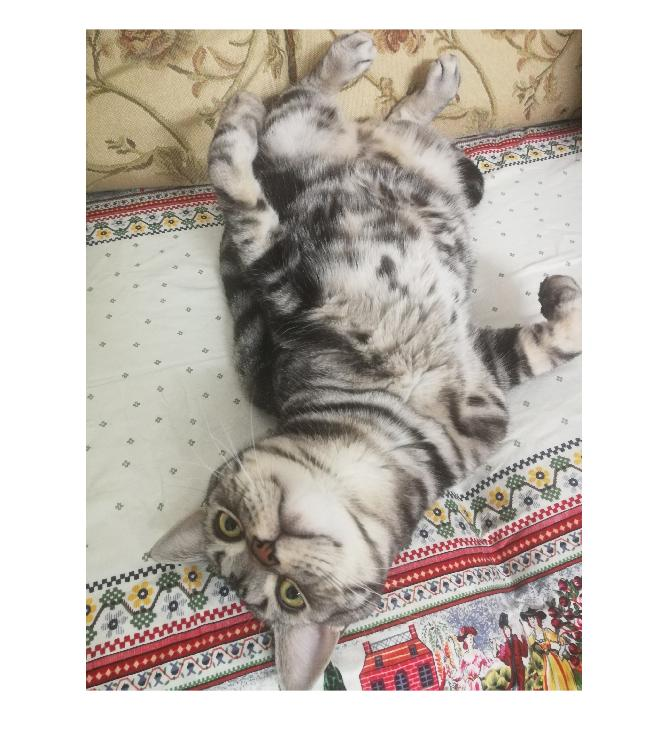
\includegraphics[width=0.5\textwidth]{./img/cat.jpg}
    \caption{可爱的小猫咪}
    \label{Fig.cat}
\end{figure}

\subsection{多张子图}
图\ref{Fig.filt}是被玩坏了的小猫咪。
\begin{figure}[H]
    \centering
    \subfigure[高斯滤波]{
        \label{Fig.Gfilt}
        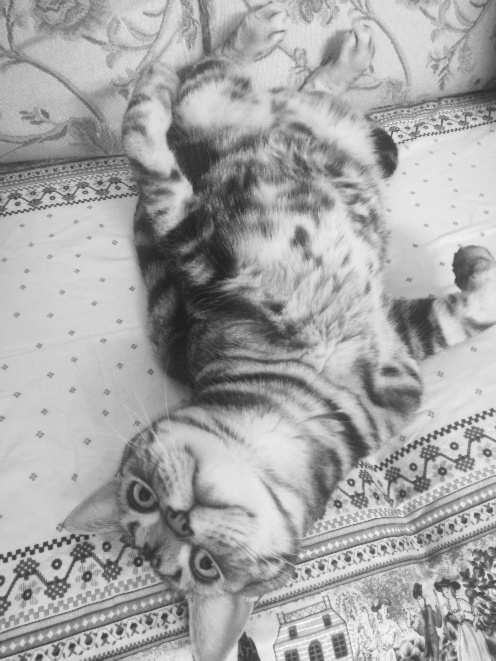
\includegraphics[width=0.3\textwidth,]{./img/cat_Guassian.jpg}}
    \subfigure[梯度滤波]{
        \label{Fig.Sfilt}
        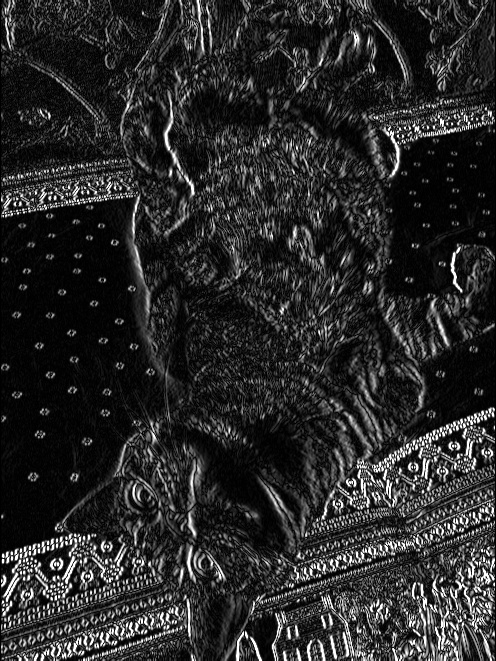
\includegraphics[width=0.3\textwidth]{./img/cat_Sobel.jpg}}
    \caption{基于梯度滤波的边缘检测}
    \label{Fig.filt}
\end{figure}


\section{表格}
\subsection{基础表格}
表\ref{Tab.GPA}是一张最普通的表格。人物、成绩纯属虚构。
\begin{table}[H]
    \centering
    \caption{某某班级成绩表}
    \label{Tab.GPA}
    \begin{tabular}{|c|c|c|c|}
        \hline
        学号     & 姓名   & 绩点 & 排名 \\
        \hline
        04000001 & 李雷   & 4.101 & 1 \\
        \hline
        04000002 & 韩梅梅 & 4.061 & 2 \\
        \hline
        04000003 & 李雷梅 & 3.999 & 3 \\
        \hline
    \end{tabular}
\end{table}

\subsection{合并单元格}
\subsubsection{纵向合并}
表\ref{Tab.portTop}是某次实验里贴过来的。
\begin{table}[H]
    \centering
    \caption{顶层模块端口定义}
    \label{Tab.portTop}
    \begin{tabular}{|c|c|c|}
        \hline
        \multirow{3}*{输入端口} & CLK0 & 时钟 \\ \cline{2-3}
        & ena0 & 使能 \\ \cline{2-3}
        & rst0 & 清零 \\ \hline
        \multirow{2}*{输出端口} & led & 显示 \\ \cline{2-3}
        & cout0 & 进位标志 \\ \hline
    \end{tabular}
\end{table}

\subsubsection{横向合并}
表\ref{Tab.score}展示了上面几个虚构的同学“四大名补”的分数。所有信息纯属虚构,如有雷同,纯属巧合。
\begin{table}[H]
    \centering
    \caption{某某班四大名补均分表}
    \label{Tab.score}
    \begin{tabular}{|c|c|c|c|c|}
        \hline
        \multirow{2}*{姓名} & \multicolumn{4}{c|}{成绩} \\
        \cline{2-5}
        & 电路 & 信号 & 模电 & 电磁场 \\
        \hline
        李雷 & 80 & 85 & 82 & 85 \\ 
        \hline
        韩梅梅 & 85 & 90 & 88 & 83 \\
        \hline
        李雷梅 & 81 & 91 & 87 & 93 \\ 
        \hline
    \end{tabular}
\end{table}

\section{算法}
算法\ref{Alg.magic}是一个神奇的算法,形象生动地展示了令人窒息的操作。
\begin{algorithm}
    \caption{神奇算法}
    \label{Alg.magic}
    \KwIn{$\bm x_{train}, \bm y_{train}, \theta$}
    \KwOut{$\bm \omega$}
    $\bm \omega \leftarrow \bm 0$\;
    $n \leftarrow 0$\;
    \While{大条件}
    {
        $J \leftarrow \|{\bm \omega \bm x_{train} - \bm y_{train}}\|_2^2$\;
        \If{小条件}
        {
            神奇的操作\;
            用神奇的方法更新$\bm \omega$\;
        }
        \Else
        {
            更神奇的操作\;
            用更神奇的方法更新$\bm \omega$\;
        }
        $n \leftarrow n + 1$\;
    }
\end{algorithm}

\section{代码}
使用Listings优雅地插入代码。代码清单\ref{imfilt_test.py}是用来产生图\ref{Fig.filt}的程序。Listings支持各种编程语言,您只需要把导言区和下面的“Python”换成其他语言即可。
\lstinputlisting[
style       =   Python,
caption     =   {基于Python和OpenCV的边缘检测实现},
label       =   {imfilt_test.py}
]{./code/imfilt_test.py}

\section{引文}
文献\cite{Goodfellow-et-al-2016}因为封面上盛开的鲜花,又叫“花书”,是深度学习的圣经。
%%%%%%%%%%%%%%%%%%%%%%%%%%%%%%%%%%%%%%%%%%%%%%%%%%%%%%%%%%%%%%%
%------------------The main article ends here-----------------%

%--------------------------References-------------------------%
\bibliography{./reference.bib}
\addcontentsline{toc}{section}{参考文献} % Add to contents

\end{document}